%###########################PRESENTACION##########################################
%Modo presentación
\documentclass[14pt]{beamer}

%Modo handout
%\documentclass[handout,compress]{beamer}
%\usepackage{pgfpages}
%\pgfpagesuselayout{4 on 1}[border shrink=1mm]

\usepackage{graphicx,pstricks}
\usepackage{beamerthemeCambridgeUS}
\usepackage{subfig}
\usepackage{tikz}
\usepackage{amsmath}
\usepackage{hyperref}

\graphicspath{{G:/My Drive/FIGURAS/}}
\setbeamercovered{transparent}

\title[GIS - CRS]{ANÁLISIS GEOESPACIAL}
\author[Edier Aristizábal]{Edier V. Aristizábal G.}
\institute{\emph{evaristizabalg@unal.edu.co}}
\date{\tiny{(Versión:\today)}}
\usepackage{textpos}

\addtobeamertemplate{headline}{}{%
	\begin{textblock*}{2mm}(.9\textwidth,0cm)
	\hfill
\includegraphics[height=1cm]{un}
	\end{textblock*}}
			
%############################INICIO#############################################
\begin{document}
\begin{frame}
\titlepage
\centering
	
\includegraphics[width=5cm]{unal}\hspace*{4.75cm}~%
   	
\includegraphics[width=2cm]{logo3}
\end{frame}
 %#############################SLIDE\begin{frame}
\begin{frame}
\frametitle{\emph{The Earth}}
  \begin{figure}
    \centering
    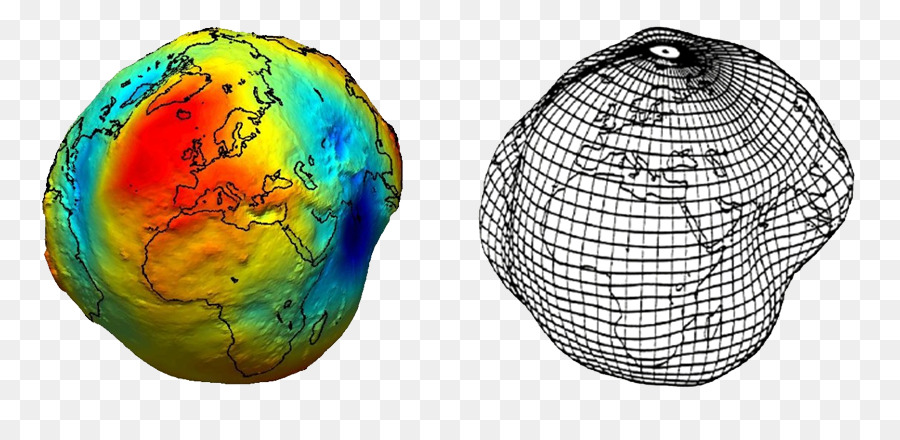
\includegraphics[height=.7\textheight]{earth}
   \end{figure}
\end{frame}
%################################SLIDE
\begin{frame}
\frametitle{Geoide}
  \begin{figure}
    \centering
    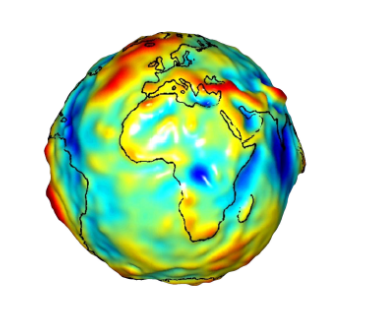
\includegraphics[height=.7\textheight]{geoide}
    %\caption{This is the caption.}
  \end{figure}
\end{frame}
%################################SLIDE
\begin{frame}
\frametitle{Elipsoide}
\framesubtitle{WGS84}
  \begin{figure}
    \centering
    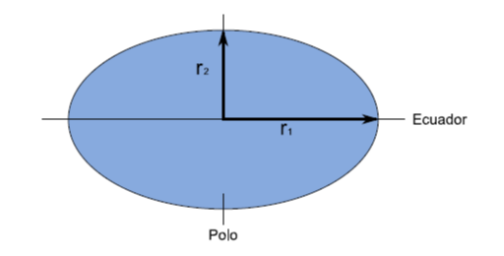
\includegraphics[height=.7\textheight]{elipsoide}
    %\caption{This is the caption.}
  \end{figure}
\end{frame}
%################################SLIDE
\begin{frame}
\frametitle{Elipsoide \& Geoide}
\framesubtitle{Datum geodésico}
  \begin{figure}
    \centering
    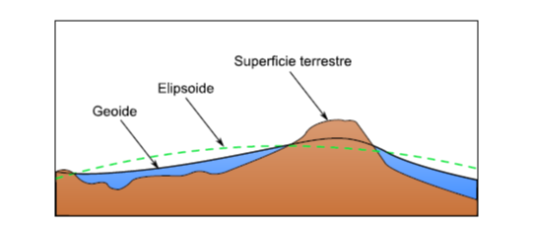
\includegraphics[height=.6\textheight]{geoide2}
    %\caption{This is the caption.}
  \end{figure}
\end{frame}
%################################SLIDE
\begin{frame}
\frametitle{Coordenadas Geográficas}
%\framesubtitle{}
  \begin{figure}
    \centering
    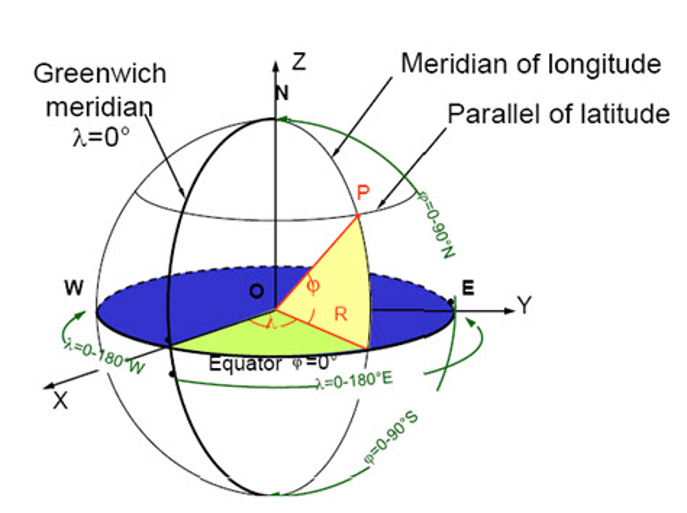
\includegraphics[height=.7\textheight]{coordenadas}
    %\caption{This is the caption.}
  \end{figure}
\end{frame}
%################################SLIDE
\begin{frame}
\frametitle{Proyección a Coordenadas Planas}
\framesubtitle{\emph{You can’t represent Earth’s surface in two dimensions without distortion}}
\scriptsize{Similarly, a map projection is a method by which cartographers translates a sphere or globe into a two-dimensional representation. In other words, a map projection systematically renders a 3D ellipsoid (or spheroid) of Earth to a 2D map surface. Because you can’t display 3D surfaces perfectly in two dimensions, distortions always occur. For example, map projections distort distance, direction, scale and area.}
  \begin{figure}
    \centering
    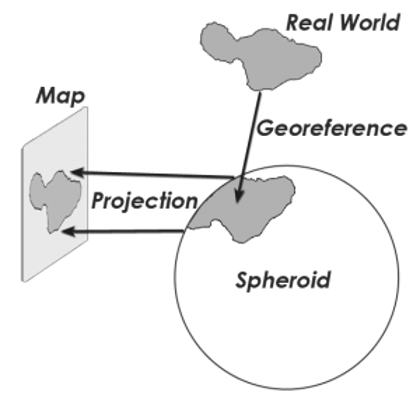
\includegraphics[height=.6\textheight]{projec}
    %\caption{This is the caption.}
  \end{figure}
\end{frame}
%################################SLIDE
\begin{frame}
\frametitle{Proyección Cartográfica}
%\framesubtitle{}
  \begin{figure}
    \centering
    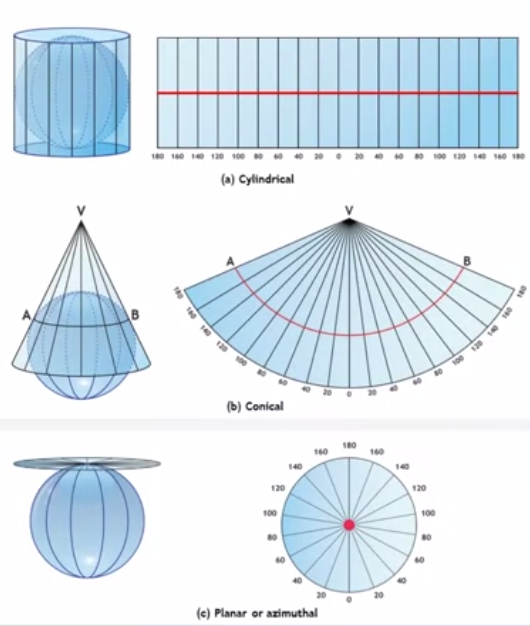
\includegraphics[height=.8\textheight]{proy}
    %\caption{This is the caption.}
  \end{figure}
\end{frame}
%################################SLIDE
\begin{frame}
\frametitle{Proyección Cilíndrica}
%\framesubtitle{}
  \begin{figure}
    \centering
    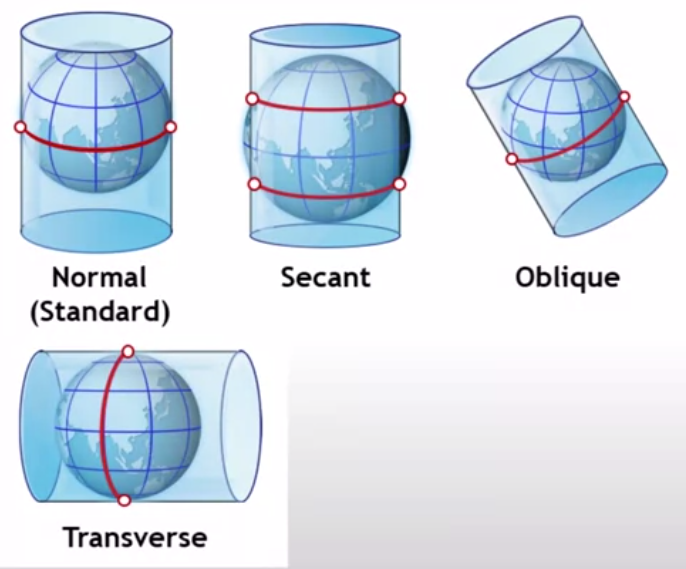
\includegraphics[height=.8\textheight]{cilindrica}
    %\caption{This is the caption.}
  \end{figure}
\end{frame}
%################################SLIDE
\begin{frame}
\frametitle{Proyección Cónica}
%\framesubtitle{}
  \begin{figure}
    \centering
    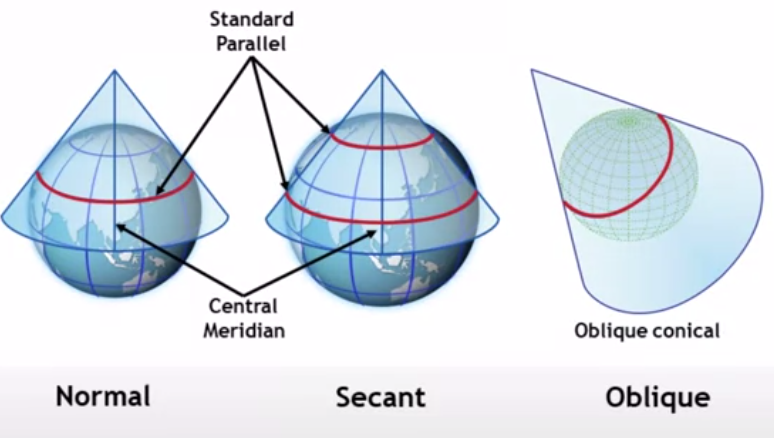
\includegraphics[height=.8\textheight]{conical}
    %\caption{This is the caption.}
  \end{figure}
\end{frame}
%################################SLIDE
\begin{frame}
\frametitle{Proyección Planar}
%\framesubtitle{}
  \begin{figure}
    \centering
    \includegraphics[height=.8\textheight]{Planar}
    %\caption{This is the caption.}
  \end{figure}
\end{frame}
%################################SLIDE
\begin{frame}
\frametitle{Proyección Cartográfica}
%\framesubtitle{}
  \begin{figure}
    \centering
    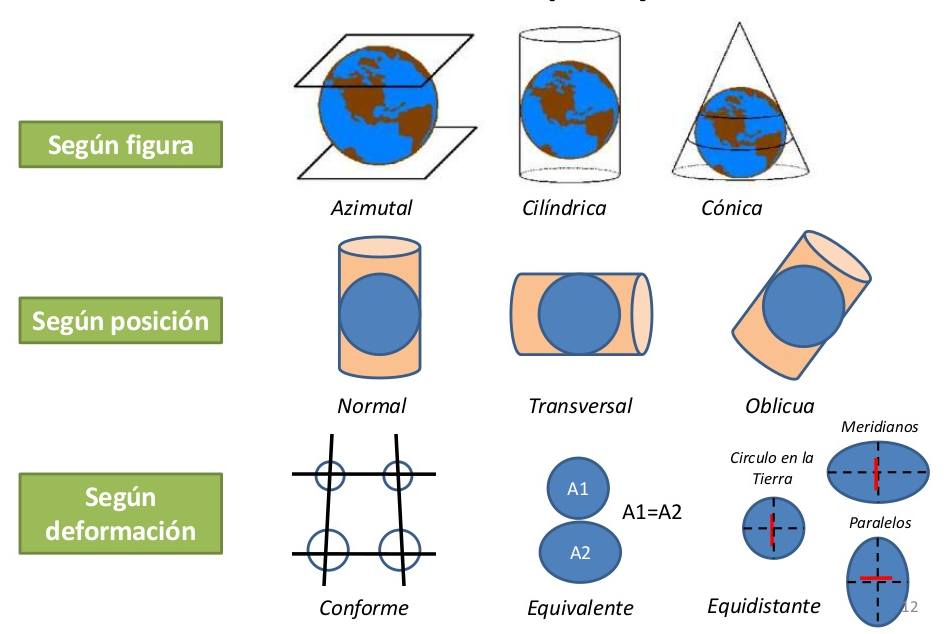
\includegraphics[height=.7\textheight]{proye}
    %\caption{This is the caption.}
  \end{figure}
\end{frame}
%################################SLIDE
\begin{frame}
\frametitle{Universal Transversal Mercator (UTM)}
%\framesubtitle{}
  \begin{figure}
    \centering
    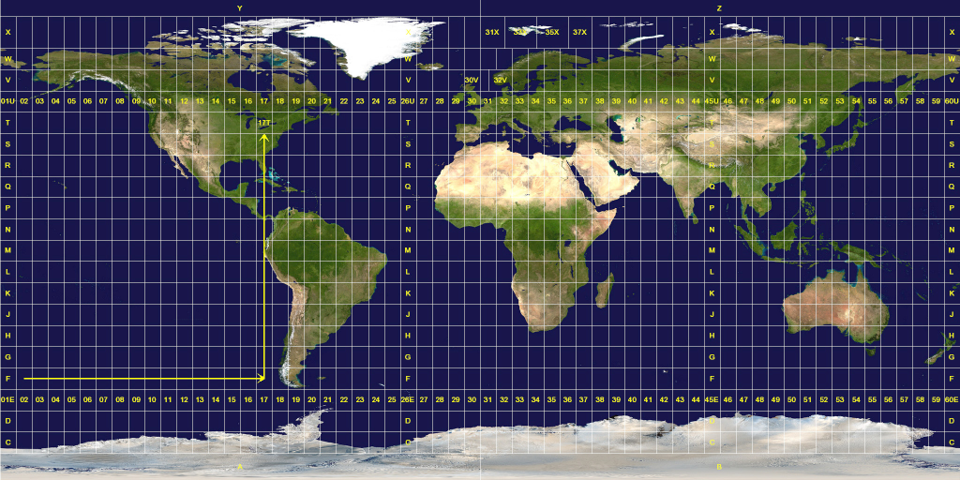
\includegraphics[height=.7\textheight]{utm}
    %\caption{This is the caption.}
  \end{figure}
\end{frame}
%################################SLIDE
\begin{frame}
\frametitle{Proyección Conforme de Gauss}
%\framesubtitle{}
  \begin{figure}
    \centering
    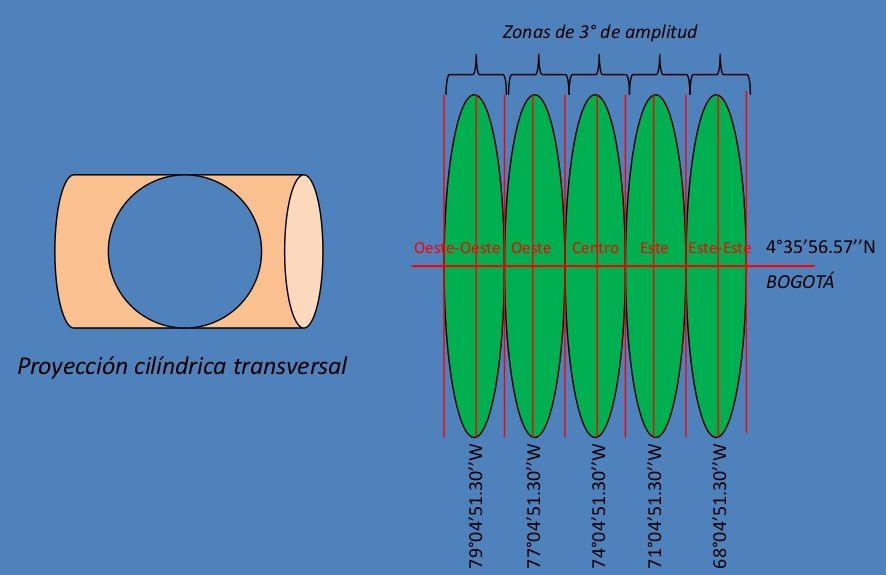
\includegraphics[height=.8\textheight]{gauss}
    %\caption{This is the caption.}
  \end{figure}
\end{frame}
%################################SLIDE
\begin{frame}
\frametitle{Proyección Conforme de Gauss}
%\framesubtitle{}
  \begin{figure}
    \centering
    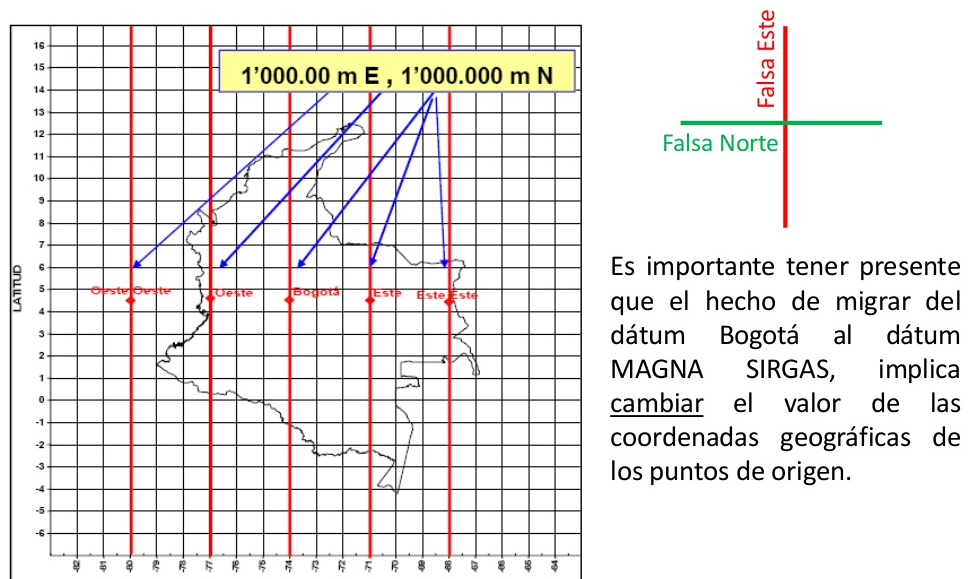
\includegraphics[height=.7\textheight]{gauss2}
    %\caption{This is the caption.}
  \end{figure}
\end{frame}
%################################SLIDE
\begin{frame}
\frametitle{Spatial Reference System Identifier (SRID)}
\scriptsize{Un SRID, Identificador de Referencia Espacial, es un identificador estándar único que hace referencia a un Sistema de Coordenadas concreto. Cada código, por tanto, se asocia de forma exclusiva a un Sistema de Coordenadas.}
%\framesubtitle{}
  \begin{figure}
    \centering
    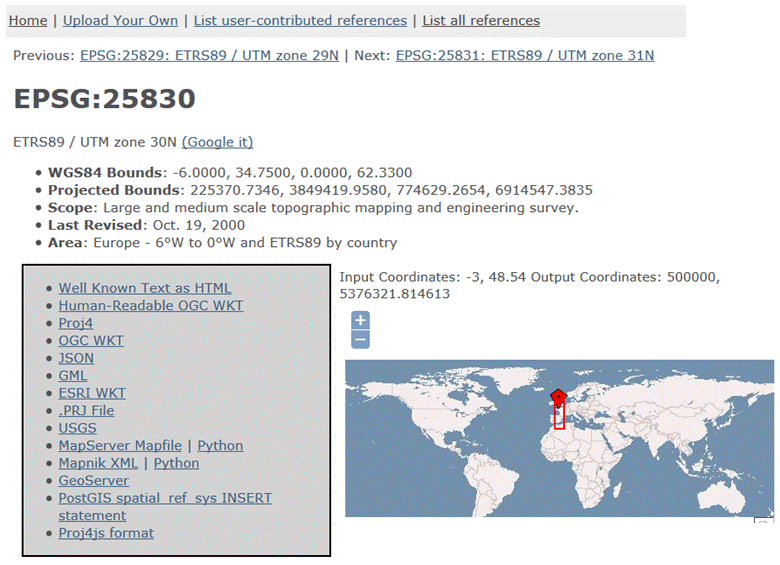
\includegraphics[height=.6\textheight]{epsg}
    %\caption{This is the caption.}
  \end{figure}
\url{https://www.spatialreference.org/}
\end{frame}
%################################SLIDE
\begin{frame}
\frametitle{The True Size of...}
\framesubtitle{\url{https://thetruesize.com}}
  \begin{figure}
  \centering
    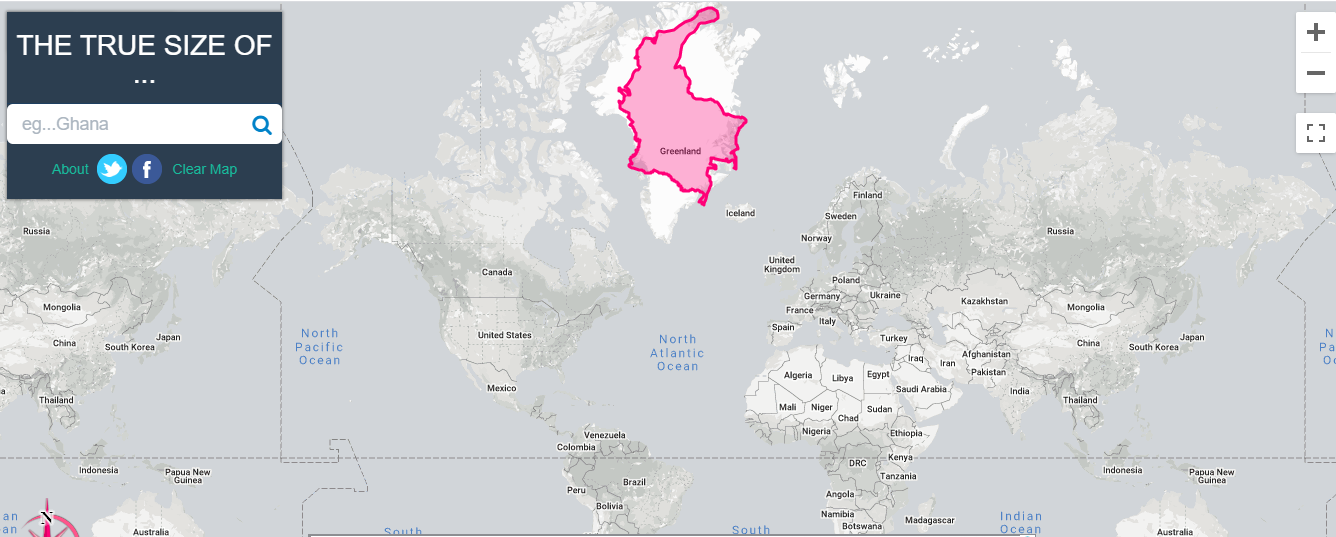
\includegraphics[height=0.8\textheight]{truesize}
\tiny{}
  \end{figure}
\end{frame}
%%%%%%%%%%%%%%%%%%%%%%%%%%%%%%%%%%%%%%%%%%%%%%%%%%%%%%%%%%%
\end{document}